
\subsection{Caso de estudio: el casco de referencia}\label{sec:casco}

Para que la matemática no quede en el aire, todo el desarrollo que sigue se hace con una fotografía real y con
los números que produce el programa: el casco que el profesor pidió usar como objeto de prueba (figura~\ref{fig:casco-entrada}).
La foto se subió con el botón \textbf{Subir foto} de la página (procesamiento bajo) y los valores de esta sección
salen de ejecutar cada paso por separado (\texttt{experimentos/casco\_paso\_a\_paso.py}); el modelo que aparece en la
pestaña del escáner (figura~\ref{fig:visor-bajo}) coincide con ellos, con $N=65\,314$ vértices y $M=130\,624$ caras.

\begin{figure}[htbp]
\centering
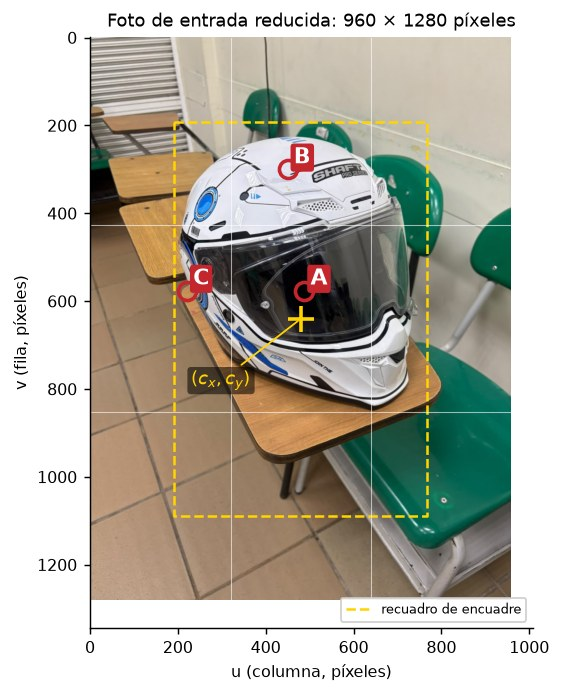
\includegraphics[height=8.2cm]{casco_entrada.jpg}
\hfill
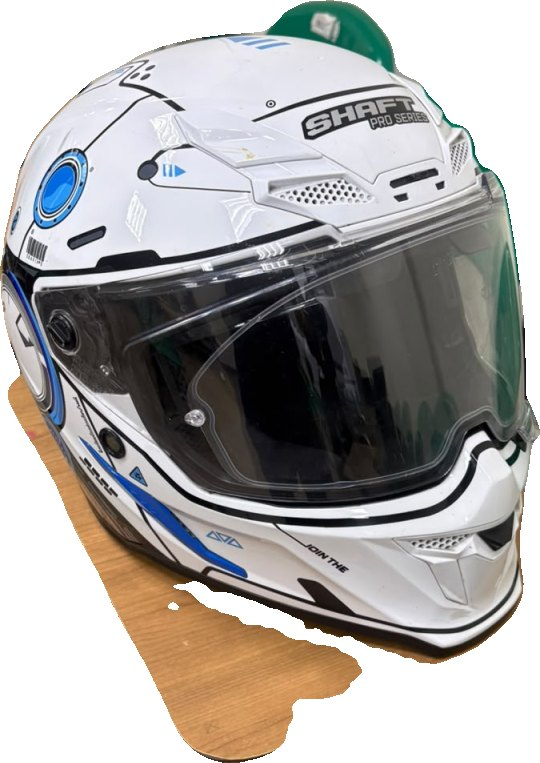
\includegraphics[height=8.2cm]{casco_recorte.jpg}
\caption{Foto de referencia reducida a $960\times1280$ píxeles, con los ejes $u$ (columna) y $v$ (fila), el recuadro de
encuadre, el centro de la imagen $(c_x,c_y)$ y los tres píxeles A, B y C que se siguen en las cuentas (izquierda); objeto
recortado por la máscara (derecha).}
\label{fig:casco-entrada}
\end{figure}

\subsection{Matriz de la cámara y su inversa con los valores del casco}\label{sec:casco-camara}

El ángulo de visión horizontal que usa el programa es $\alpha=65^\circ$ y la foto mide $W=960$ píxeles de ancho
y $H=1280$ de alto. La distancia focal en píxeles y el centro de la imagen son
\begin{align*}
f &= \frac{W/2}{\tan(\alpha/2)}=\frac{480}{\tan(32{,}5^\circ)}=\frac{480}{0{,}63707}=753{,}449\ \text{píxeles},\\
c_x&=\frac{W}{2}=480,\qquad c_y=\frac{H}{2}=640 .
\end{align*}
Con ellos la matriz de la cámara y su determinante son
\begin{equation}
K=\begin{pmatrix} 753{,}449 & 0 & 480 \\ 0 & 753{,}449 & 640 \\ 0 & 0 & 1 \end{pmatrix},\qquad \det K=f\cdot f\cdot1=f^2=567\,685{,}5\neq0,
\end{equation}
así que $K$ es invertible. Su inversa se calcula con Gauss--Jordan (sección «\nameref{sec:inversa}»), con solo tres
operaciones entre filas, porque $K$ ya es triangular:
Se parte de la matriz aumentada $[K\mid I]$:
\begin{equation*}
\left(\begin{array}{ccc|ccc} 753{,}449 & 0 & 480 & 1 & 0 & 0\\ 0 & 753{,}449 & 640 & 0 & 1 & 0\\ 0&0&1&0&0&1\end{array}\right).
\end{equation*}
Se resta $c_x$ veces la fila 3 a la fila 1 y $c_y$ veces la fila 3 a la fila 2 ($F_1\leftarrow F_1-c_xF_3$, $F_2\leftarrow F_2-c_yF_3$):
\begin{equation*}
\left(\begin{array}{ccc|ccc} 753{,}449 & 0 & 0 & 1 & 0 & -480\\ 0 & 753{,}449 & 0 & 0 & 1 & -640\\ 0&0&1&0&0&1\end{array}\right).
\end{equation*}
Y se dividen las filas 1 y 2 entre $f$ ($F_1\leftarrow F_1/f$, $F_2\leftarrow F_2/f$):
\begin{equation*}
\left(\begin{array}{ccc|ccc} 1&0&0& 0{,}001327 & 0 & -0{,}637070\\ 0&1&0& 0 & 0{,}001327 & -0{,}849427\\ 0&0&1&0&0&1\end{array}\right).
\end{equation*}
Entonces
\begin{equation}
K^{-1}=\begin{pmatrix} 0{,}001327 & 0 & -0{,}637070 \\ 0 & 0{,}001327 & -0{,}849427 \\ 0 & 0 & 1 \end{pmatrix} .
\end{equation}
La comprobación numérica $KK^{-1}=I$ da
\begin{equation}
KK^{-1}=\begin{pmatrix} 753{,}449 & 0 & 480 \\ 0 & 753{,}449 & 640 \\ 0 & 0 & 1 \end{pmatrix}\begin{pmatrix} 0{,}001327 & 0 & -0{,}637070 \\ 0 & 0{,}001327 & -0{,}849427 \\ 0 & 0 & 1 \end{pmatrix}=\begin{pmatrix} 1 & 0 & 0 \\ 0 & 1 & 0 \\ 0 & 0 & 1 \end{pmatrix} .
\end{equation}

\subsection{La máscara $M$ del casco}\label{sec:casco-mascara}

La red U$^2$-Net entrega para cada píxel un valor $\alpha_{vu}\in[0,255]$; la máscara es la matriz de $1280\times960$ entradas
\begin{equation}
M_{vu}=\begin{cases}1&\text{si }\alpha_{vu}>127,\\0&\text{si no,}\end{cases}
\end{equation}
que luego se limpia (se quitan puntos sueltos, se rellenan huecos y se conserva la región conectada que más se
superpone con el recuadro). Para el casco, la suma de las entradas de $M$ es
$\sum M_{vu}=293\,960$ píxeles, que es el 23{,}92\,\% de los $1\,228\,800$ píxeles de la foto, y la región ocupa las columnas
$u\in[204,743]$ y las filas $v\in[191,953]$ (una caja de $540\times763$ píxeles). Cada uno de esos píxeles
será un punto del espacio.

\subsection{Profundidad del casco: de la disparidad a $Z$}\label{sec:casco-profundidad}

Para cada píxel con $M_{vu}=1$ se calculan cuatro números (las ecuaciones del Paso~2 de la metodología). Con los
valores globales $d_{\max}=257{,}814$ píxeles (la mayor distancia al borde de la silueta),
$\text{mm/px}=Z_0/f=400/753{,}449=0{,}5309$ y $R=d_{\max}\cdot\text{mm/px}=136{,}871$ mm, y con
$D_{\text{borde}}=3{,}5367$ y $D_{\text{alto}}=5{,}8436$ (mediana de la disparidad en el borde y percentil 99 dentro del casco),
el píxel A se calcula así:
\begin{align*}
s&=\frac{d}{d_{\max}}=\frac{213{,}327}{257{,}814}=0{,}82745,\\
p(s)&=\sqrt{1-(1-s)^2}=\sqrt{1-(0{,}17255)^2}=0{,}98500,\\
r&=\frac{D-D_{\text{borde}}}{D_{\text{alto}}-D_{\text{borde}}}=\frac{5{,}3068-3{,}5367}{5{,}8436-3{,}5367}=0{,}76731,\\
h&=0{,}75\,R\,(0{,}7\,r+0{,}3\,p)=0{,}75\cdot136{,}871\cdot0{,}83262=85{,}47\ \text{mm}.
\end{align*}
El valor guardado, $h=85{,}44$ mm, es el de la fórmula después de un suavizado gaussiano que quita escalones. Con
$g=0{,}10\,R=13{,}687$ mm (medio grosor):
\begin{align*}
Z_{\text{frente}}&=Z_0-g-h=400-13{,}687-85{,}44=300{,}87\ \text{mm},\\
Z_{\text{atrás}}&=Z_0+g+0{,}6\,h=400+13{,}687+0{,}6\cdot85{,}44=464{,}95\ \text{mm}.
\end{align*}
El cuadro~\ref{tab:casco-prof} reúne los tres píxeles, la figura~\ref{fig:casco-etapas} muestra las matrices completas
($I$, $M$, $D$ y $Z_{\text{frente}}$) y la figura~\ref{fig:casco-perfil} sigue la fila del píxel A.

\begin{table}[htbp]
\caption{Profundidad de los tres píxeles de ejemplo (longitudes en mm)}
\label{tab:casco-prof}
\centering\small
\begin{tabular}{@{}lrrrrrrrr@{}}
\toprule
Píxel & $d$ (px) & $s$ & $p(s)$ & $D$ & $r$ & $h$ & $Z_{\text{frente}}$ & $Z_{\text{atrás}}$ \\
\midrule
A & 213{,}33 & 0{,}8274 & 0{,}9850 & 5{,}3068 & 0{,}7673 & 85{,}44 & 300{,}87 & 464{,}95 \\
B & 77{,}00 & 0{,}2987 & 0{,}7128 & 5{,}3516 & 0{,}7867 & 78{,}37 & 307{,}94 & 460{,}71 \\
C & 5{,}60 & 0{,}0217 & 0{,}2073 & 2{,}7236 & 0{,}0000 & 7{,}17 & 379{,}14 & 417{,}99 \\
\bottomrule
\end{tabular}
\end{table}

\begin{figure}[htbp]
\centering
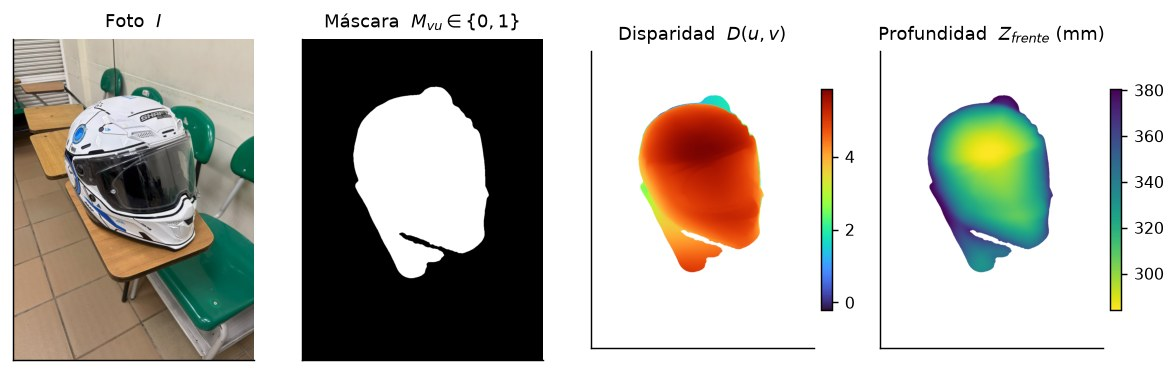
\includegraphics[width=\linewidth]{casco_etapas.jpg}
\caption{Matrices del casco: foto $I$, máscara $M$, disparidad $D(u,v)$ de la red y profundidad $Z_{\text{frente}}(u,v)$
en milímetros (solo dentro de la máscara).}
\label{fig:casco-etapas}
\end{figure}

\begin{figure}[htbp]
\centering
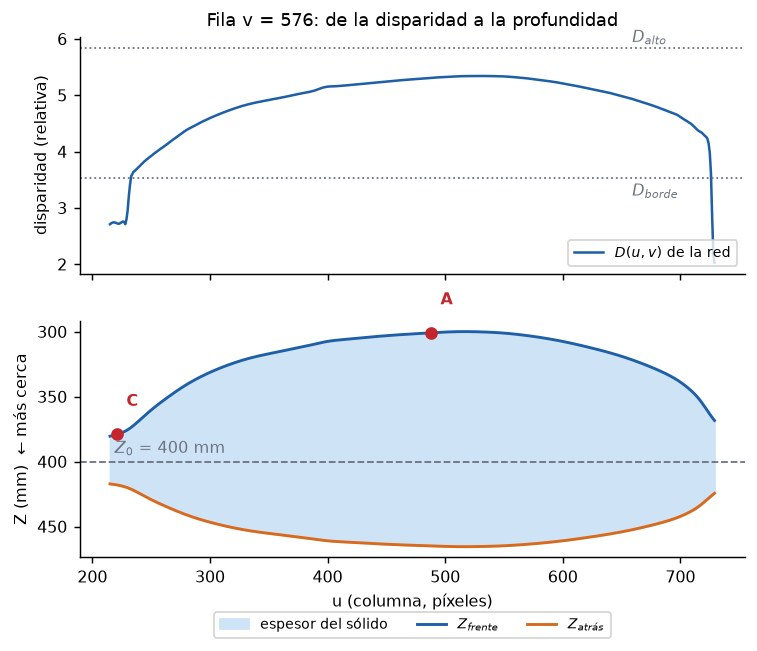
\includegraphics[width=0.82\linewidth]{casco_perfil.jpg}
\caption{Fila $v=576$ (la del píxel A y el C): la disparidad $D$ (arriba) se convierte en las profundidades $Z_{\text{frente}}$ y
$Z_{\text{atrás}}$ (abajo); el espesor del sólido es la diferencia entre ambas.}
\label{fig:casco-perfil}
\end{figure}

\subsection{Retroproyección del casco: de píxeles a puntos 3D}\label{sec:casco-retro}

\paragraph{Un píxel.} El píxel A se escribe en coordenadas homogéneas, $\vect{p}_A=(u,v,1)^T=\begin{pmatrix} 488 \\ 576 \\ 1 \end{pmatrix}$, y su rayo es
\begin{equation}
\vect{r}_A=K^{-1}\vect{p}_A=\begin{pmatrix} 0{,}001327 & 0 & -0{,}637070 \\ 0 & 0{,}001327 & -0{,}849427 \\ 0 & 0 & 1 \end{pmatrix}\begin{pmatrix} 488 \\ 576 \\ 1 \end{pmatrix}=\begin{pmatrix} 0{,}010618 \\ -0{,}084943 \\ 1 \end{pmatrix} .
\end{equation}
El punto 3D es el rayo multiplicado por la profundidad $Z_{\text{frente}}=300{,}87$ mm:
\begin{equation}
\vect{P}_A=Z\,\vect{r}_A=300{,}87\cdot\begin{pmatrix} 0{,}010618 \\ -0{,}084943 \\ 1 \end{pmatrix}=\begin{pmatrix} 3{,}195 \\ -25{,}557 \\ 300{,}871 \end{pmatrix}\ \text{mm}.
\end{equation}
Es decir, A está a $3{,}19$ mm a la derecha, $25{,}56$ mm arriba del eje de la cámara y a $300{,}87$ mm al frente.
Para comprobarlo se proyecta de nuevo: $K\vect{P}_A=\begin{pmatrix} 146825{,}0 \\ 173301{,}6 \\ 300{,}9 \end{pmatrix}=Z\,\vect{p}_A$, y al dividir entre $Z$ se recupera el píxel $(488,576,1)$.

\paragraph{Por qué hace falta $Z$: el sistema $2\times3$.} Las dos ecuaciones de la proyección, con $\vect{P}=(X,Y,Z)^T$ desconocido y
el píxel A conocido, forman el sistema homogéneo
\begin{equation}
\begin{pmatrix}f&0&c_x-u\\0&f&c_y-v\end{pmatrix}\begin{pmatrix}X\\Y\\Z\end{pmatrix}=
\begin{pmatrix} 753{,}449 & 0 & -8 \\ 0 & 753{,}449 & 64 \end{pmatrix}\begin{pmatrix}X\\Y\\Z\end{pmatrix}=\begin{pmatrix}0\\0\end{pmatrix}.
\end{equation}
Su matriz tiene rango $2$ y hay $3$ incógnitas, así que queda una variable libre. Al despejar:
$X=\tfrac{u-c_x}{f}Z=0{,}010618\,Z$ y $Y=\tfrac{v-c_y}{f}Z=-0{,}084943\,Z$, es decir, toda la solución es la recta
$\vect{P}=Z\,(0{,}010618,\,-0{,}084943,\,1)^T=Z\,\vect{r}_A$: el rayo. El espacio nulo de la matriz es justamente el vector $\vect{r}_A$ que dio $K^{-1}\vect{p}_A$.

\paragraph{Vectores de los rayos.} La longitud del rayo A es $\lVert\vect{r}_A\rVert=1{,}00366$ y su ángulo con el eje óptico es
$\arctan\sqrt{(0{,}010618)^2+(-0{,}084943)^2}=4{,}893^\circ$. El ángulo entre los rayos de A y C sale del producto punto:
\begin{equation}
\cos\theta=\frac{\vect{r}_A\cdot\vect{r}_C}{\lVert\vect{r}_A\rVert\,\lVert\vect{r}_C\rVert}=
\frac{1{,}00357}{1{,}00366\cdot1{,}06084}=0{,}94256\ \Rightarrow\ \theta=19{,}51^\circ .
\end{equation}

\paragraph{Muchos píxeles a la vez.} En el programa no se calcula píxel por píxel. Para cinco píxeles del casco, repartidos
a lo largo de la máscara, se apilan como columnas de una matriz $H$ de $3\times5$ y se multiplica una sola vez:
\begin{equation}
H=\begin{pmatrix} 530 & 662 & 537 & 723 & 443 \\ 191 & 406 & 549 & 696 & 953 \\ 1 & 1 & 1 & 1 & 1 \end{pmatrix},
\end{equation}
\begin{equation}
K^{-1}H=\begin{pmatrix} 0{,}0664 & 0{,}2416 & 0{,}0757 & 0{,}3225 & -0{,}0491 \\ -0{,}5959 & -0{,}3106 & -0{,}1208 & 0{,}0743 & 0{,}4154 \\ 1 & 1 & 1 & 1 & 1 \end{pmatrix} .
\end{equation}
Multiplicar a la derecha por la matriz diagonal $\operatorname{diag}(Z_1,\dots,Z_5)$, con
$(Z_1,\dots,Z_5)=\begin{pmatrix} 380{,}39 & 312{,}13 & 298{,}65 & 354{,}57 & 335{,}32 \end{pmatrix}$ mm, escala cada columna por su profundidad:
\begin{equation}
P=K^{-1}H\,\operatorname{diag}(Z_1,\dots,Z_5)=\begin{pmatrix} 25{,}24 & 75{,}40 & 22{,}59 & 114{,}36 & -16{,}47 \\ -226{,}68 & -96{,}94 & -36{,}07 & 26{,}35 & 139{,}30 \\ 380{,}39 & 312{,}13 & 298{,}65 & 354{,}57 & 335{,}32 \end{pmatrix}\ \text{mm}.
\end{equation}
Con los $32\,657$ nodos de la malla el procedimiento es el mismo, con una matriz $H$ de $3\times32\,657$.

\subsection{Cambio de ejes: del sistema de la cámara al del objeto}\label{sec:casco-ejes}

Los puntos $\vect{P}$ están en los ejes de la cámara ($X$ a la derecha, $Y$ hacia abajo, $Z$ hacia adelante). El visor 3D usa los ejes
del objeto ($x$ a la derecha, $y$ hacia arriba, $z$ hacia el observador). Se pasa de uno a otro con una traslación al centro del
objeto, $\vect{c}$ (el punto medio de la caja que contiene a todos los vértices), y una rotación de $180^\circ$ alrededor del eje $x$:
\begin{equation}
\vect{p}=R_o(\vect{P}-\vect{c}),\qquad R_o=\begin{pmatrix} 1 & 0 & 0 \\ 0 & -1 & 0 \\ 0 & 0 & -1 \end{pmatrix},\qquad \vect{c}=\begin{pmatrix} -3{,}354 \\ -36{,}101 \\ 379{,}535 \end{pmatrix}\ \text{mm}.
\end{equation}
$R_o$ es una rotación ($R_o^TR_o=I$ y $\det R_o=1$), su inversa es su transpuesta y, como es diagonal, $R_o^{-1}=R_o^T=R_o$. Para el píxel A:
\begin{equation}
\vect{p}_A=R_o\left(\begin{pmatrix} 3{,}195 \\ -25{,}557 \\ 300{,}871 \end{pmatrix}-\begin{pmatrix} -3{,}354 \\ -36{,}101 \\ 379{,}535 \end{pmatrix}\right)=R_o\begin{pmatrix} 6{,}549 \\ 10{,}544 \\ -78{,}664 \end{pmatrix}=\begin{pmatrix} 6{,}549 \\ -10{,}544 \\ 78{,}664 \end{pmatrix}\ \text{mm}.
\end{equation}

\paragraph{Con una sola matriz de $4\times4$.} La traslación y la rotación se pueden juntar en una matriz homogénea de $4\times4$ que actúa sobre
el punto con un $1$ agregado, $(\vect{P},1)$ (coordenadas homogéneas, igual que el píxel $(u,v,1)$):
\begin{equation}
\begin{pmatrix}\vect{p}\\1\end{pmatrix}=\mathcal{M}_o\begin{pmatrix}\vect{P}\\1\end{pmatrix},\qquad
\mathcal{M}_o=\begin{pmatrix}R_o&-R_o\vect{c}\\\vect{0}^{T}&1\end{pmatrix}=\begin{pmatrix} 1 & 0 & 0 & 3{,}354 \\ 0 & -1 & 0 & -36{,}101 \\ 0 & 0 & -1 & 379{,}535 \\ 0 & 0 & 0 & 1 \end{pmatrix} .
\end{equation}
Su determinante es $\det\mathcal{M}_o=\det R_o=1$ (una matriz de rotación y traslación no cambia volúmenes), y su inversa se obtiene por bloques,
porque $-R_o^{T}(-R_o\vect{c})=\vect{c}$:
\begin{equation}
\mathcal{M}_o^{-1}=\begin{pmatrix}R_o^{T}&\vect{c}\\\vect{0}^{T}&1\end{pmatrix}=\begin{pmatrix} 1 & 0 & 0 & -3{,}354 \\ 0 & -1 & 0 & -36{,}101 \\ 0 & 0 & -1 & 379{,}535 \\ 0 & 0 & 0 & 1 \end{pmatrix},\qquad
\mathcal{M}_o\,\mathcal{M}_o^{-1}=\begin{pmatrix} 1 & 0 & 0 & 0 \\ 0 & 1 & 0 & 0 \\ 0 & 0 & 1 & 0 \\ 0 & 0 & 0 & 1 \end{pmatrix}=I_4 .
\end{equation}
Con el píxel A, $\mathcal{M}_o(\vect{P}_A,1)=\begin{pmatrix} 6{,}549 \\ -10{,}544 \\ 78{,}664 \\ 1 \end{pmatrix}=(\vect{p}_A,1)$, y al revés, $\mathcal{M}_o^{-1}(\vect{p}_A,1)=\begin{pmatrix} 3{,}195 \\ -25{,}557 \\ 300{,}871 \\ 1 \end{pmatrix}=(\vect{P}_A,1)$: la inversa
devuelve el punto a los ejes de la cámara.

La figura~\ref{fig:casco-corte} muestra un corte lateral de los puntos del frente y de la parte de atrás y los rayos que los generan.

\begin{figure}[htbp]
\centering
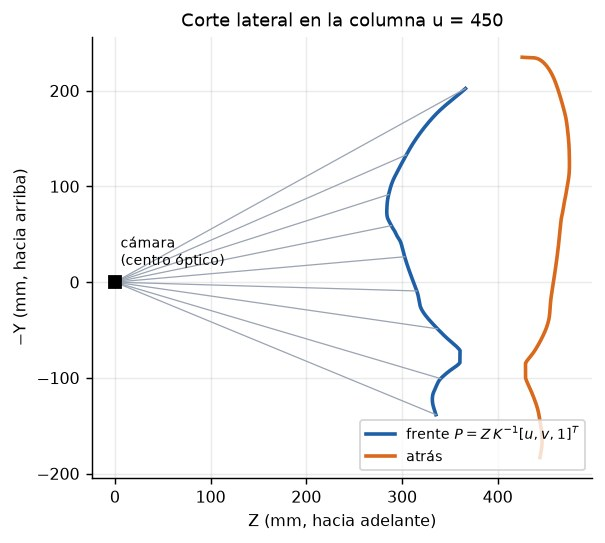
\includegraphics[width=0.78\linewidth]{casco_corte.jpg}
\caption{Corte lateral (plano $Y$--$Z$) a lo largo de la columna $u=450$: cada punto del frente está sobre el rayo de su
píxel, a la profundidad $Z_{\text{frente}}$; la parte de atrás queda a $Z_{\text{atrás}}$.}
\label{fig:casco-corte}
\end{figure}

\subsection{Construcción de la malla $V$, $F$ del casco}\label{sec:casco-malla}

Sobre la caja de $540\times763$ píxeles se coloca una rejilla con un nodo cada $3$ píxeles (el paso es $\lceil\max(540,763)/300\rceil=3$, para
tener a lo sumo 300 nodos por lado). Los nodos que caen dentro de la máscara son $32\,657$ ($\approx293\,960/9$, pues cada nodo representa
$3\times3$ píxeles). Cada uno se retroproyecta dos veces: una a $Z_{\text{frente}}$ y otra a $Z_{\text{atrás}}$, así que
$V$ tiene $2\cdot32\,657=65\,314$ filas. Las primeras filas de $V$ (en mm, ejes del objeto) y de $F$ (índices de fila de $V$) son
\begin{equation}
V=\begin{pmatrix} 29{,}062 & 190{,}855 & -0{,}855 \\ 30{,}618 & 190{,}904 & -0{,}864 \\ 32{,}170 & 190{,}719 & -0{,}891 \\ 16{,}906 & 189{,}386 & -0{,}890 \end{pmatrix}\ \text{mm},\qquad F=\begin{pmatrix} 0 & 11 & 1 \\ 1 & 12 & 2 \\ 3 & 21 & 4 \\ 4 & 22 & 5 \end{pmatrix} .
\end{equation}
Cada celda de la rejilla con sus cuatro esquinas dentro del casco se divide en dos triángulos; la parte de atrás repite los mismos
triángulos con el orden invertido, y las paredes unen el contorno. Quedan 64\,549 caras en el frente, 64\,549 atrás y 1\,526 en las
paredes: $M=130\,624$ triángulos en total.

\paragraph{Comprobación de que la malla es un sólido cerrado.} En una malla cerrada de triángulos cada arista es de dos caras, así que el número de aristas es
$E=3M/2=195\,936$. La característica de Euler de una superficie cerrada sin agujeros (como una esfera) es $\chi=V-E+F=2$; aquí
$\chi=65\,314-195\,936+130\,624=2$.

\paragraph{Un triángulo en detalle.} Se toma el triángulo $16\,135$ del frente (el más cercano al centro del casco), de la fila $F_{16\,135}=( 16260,\,16429,\,16261 )$ de $F$
(figura~\ref{fig:casco-malla-zoom}). Sus vértices, como filas de una matriz de $3\times3$, y los dos lados que salen de $\vect{p}_0$ son
\begin{equation}
\begin{pmatrix}\vect{p}_0\\\vect{p}_1\\\vect{p}_2\end{pmatrix}=\begin{pmatrix} -0{,}2174 & 0{,}4069 & 80{,}5510 \\ -0{,}2207 & -0{,}7513 & 80{,}2780 \\ 0{,}9743 & 0{,}3880 & 80{,}7058 \end{pmatrix},
\end{equation}
\begin{equation}
\vect{e}_1=\vect{p}_1-\vect{p}_0=\begin{pmatrix} -0{,}0033 \\ -1{,}1582 \\ -0{,}2729 \end{pmatrix},\qquad \vect{e}_2=\vect{p}_2-\vect{p}_0=\begin{pmatrix} 1{,}1917 \\ -0{,}0189 \\ 0{,}1548 \end{pmatrix} .
\end{equation}
Su normal es el producto cruz, que se calcula con el determinante simbólico de la regla de Sarrus:
\begin{equation}
\vect{n}=\vect{e}_1\times\vect{e}_2=\begin{vmatrix}\vect{i}&\vect{j}&\vect{k}\\ -0{,}0033&-1{,}1582&-0{,}2729\\ 1{,}1917&-0{,}0189&0{,}1548\end{vmatrix}=\begin{pmatrix} -0{,}1844 \\ -0{,}3248 \\ 1{,}3803 \end{pmatrix},
\end{equation}
y se normaliza dividiendo entre su longitud $\lVert\vect{n}\rVert=1{,}4299$:
\begin{equation}
\hat{\vect{n}}=\frac{\vect{n}}{\lVert\vect{n}\rVert}=\frac{1}{1{,}4299}\begin{pmatrix} -0{,}1844 \\ -0{,}3248 \\ 1{,}3803 \end{pmatrix}=\begin{pmatrix} -0{,}1290 \\ -0{,}2271 \\ 0{,}9653 \end{pmatrix} .
\end{equation}
Como $\hat n_z>0$, la cara mira hacia el observador (hacia $+z$), que es lo correcto para el frente. El volumen del tetraedro que forma este
triángulo con el origen es la sexta parte del determinante de la matriz de sus vértices:
\begin{equation}
\frac{1}{6}\det\begin{pmatrix}\vect{p}_0\\\vect{p}_1\\\vect{p}_2\end{pmatrix}=\frac{111{,}093}{6}=18{,}516\ \text{mm}^3 .
\end{equation}
Sumando esa cantidad sobre las $M$ caras se obtiene el volumen del casco,
$V_{\text{casco}}=\frac16\sum\det[\vect{p}_0\ \vect{p}_1\ \vect{p}_2]=9\,224\,864\ \text{mm}^3\approx9{,}22$ litros.

\begin{figure}[htbp]
\centering
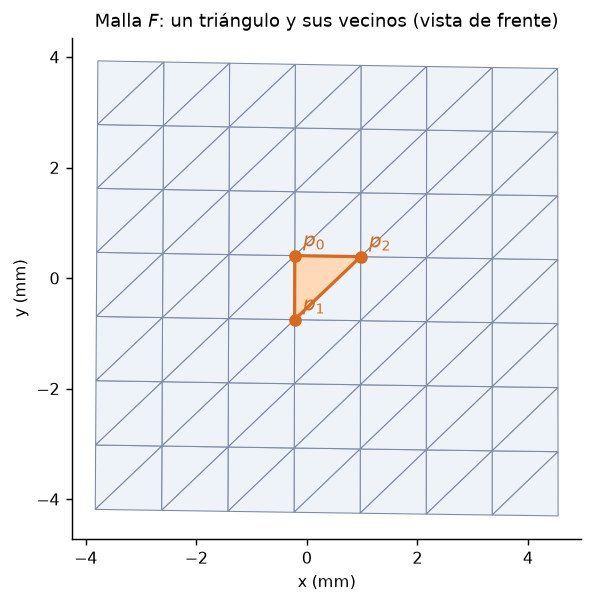
\includegraphics[width=0.62\linewidth]{casco_malla_zoom.jpg}
\caption{Zona de la malla $F$ alrededor del triángulo del ejemplo (en naranja), con sus vértices $\vect{p}_0$, $\vect{p}_1$ y $\vect{p}_2$.}
\label{fig:casco-malla-zoom}
\end{figure}

\paragraph{Resumen: matrices, vectores e inversas del proceso.} El cuadro~\ref{tab:resumen-algebra} reúne los objetos
matemáticos que aparecieron, su tamaño con el casco y cómo se usa o se invierte cada uno.

\begin{table}[htbp]
\caption{Matrices, vectores e inversas del proceso, con los valores del casco}
\label{tab:resumen-algebra}
\centering\small
\begin{tabular}{@{}p{2.3cm}p{3.0cm}p{4.2cm}p{4.0cm}@{}}
\toprule
Objeto & Tamaño & Valor en el casco & Inversa o uso \\
\midrule
$I$ (foto) & $1280\times960\times3$ & 3\,686\,400 números & el JPEG se decodifica con $C^{T}$ y $T^{-1}$ \\
$M$ (máscara) & $1280\times960$ & 293\,960 píxeles con 1 & filtra los píxeles que se retroproyectan \\
$K$ & $3\times3$ & $f=753{,}449$, $(c_x,c_y)=(480,640)$ & $K^{-1}$ con $1/f=0{,}001327$, $-c_x/f=-0{,}637070$, $-c_y/f=-0{,}849427$ \\
$\vect{r}$ (rayo) & $3\times1$ & $\vect{r}_A=(0{,}011,\,-0{,}085,\,1{,}000)^{T}$ & $K^{-1}\vect{p}$; norma $1{,}00366$ \\
$H$ & $3\times N$ & $3\times32\,657$ & $K^{-1}H\operatorname{diag}(Z)$ en un solo producto \\
$\operatorname{diag}(Z)$ & $N\times N$ & $Z\in[284,381]$ mm & inversa $\operatorname{diag}(1/Z)$ \\
$R_o$ & $3\times3$ & $\operatorname{diag}(1,-1,-1)$ & $R_o^{-1}=R_o^{T}=R_o$ \\
$V$, $F$ & $N\times3$, $M\times3$ & $65\,314$ y $130\,624$ filas & $\tfrac16\sum\det$ da el volumen: 9{,}22 L \\
$\mathcal{M}$ (alto) & $4\times4$ & rotación $R_x(90^\circ)$ & $\mathcal{M}^{-1}=\mathcal{M}^{T}$ \\
\bottomrule
\end{tabular}
\end{table}
